\documentclass{beamer}
% logo of my university
\title{Optimizing MPEG Encoding}
\author{Roel Deckers}
\institute{Uppsala University}
\begin{document}
  %key points:
  %   performance, almost-zero(tm) overhead
  %   safety (openSSL), no null pointer, no dangling pointers, no buffer overruns
  %   Compile-time, no garbage collector
  %   compatible
  %   Cargo
  %   Great and growing community. Not an easy language, but easy to get started.
  %   Quotes from people.

\begin{frame}
\titlepage
\end{frame}

\begin{frame}
  \frametitle{Why optimize MPEG?}
  \begin{itemize}
    \item{Widely used}
    \item{Many different steps}
  \end{itemize}
\end{frame}

\begin{frame}
  \frametitle{Test Machine}
  Intel i7-4750HW\\
  \begin{itemize}
    \item{Quad core, 8-threads}
    \item{32KiB L1, private}
    \item{256KiB L2, shared}
    \item{6MiB L3, shared}
    \item{128MiB L4, shared victim-cache}
  \end{itemize}
  25.6 GB/s maximum memory throughput. Measured at 20 GB/s RMW peak performance.
\end{frame}

\begin{frame}
  \frametitle{Color Conversion}
  \begin{figure}
  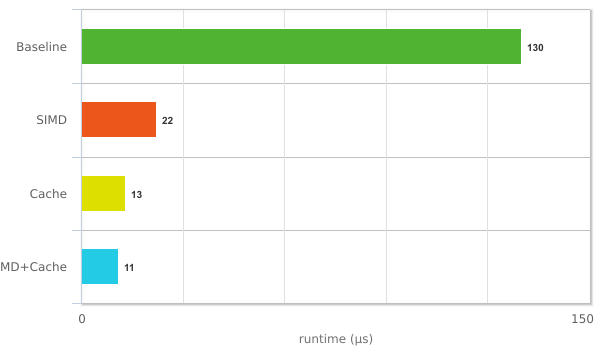
\includegraphics[width=0.9\textwidth]{images/sc}
  \caption{Single-threaded color-conversion}
  \end{figure}
\end{frame}

\begin{frame}
  \frametitle{Color Conversion}
  \begin{figure}
  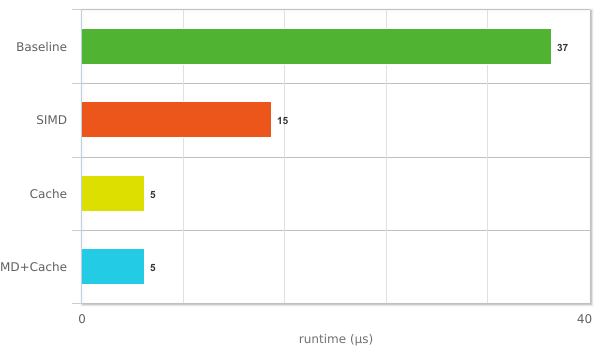
\includegraphics[width=0.9\textwidth]{images/pc}
  \caption{Multi-threaded color-conversion}
  \end{figure}
\end{frame}

\begin{frame}
  \frametitle{Downsampling}
  \begin{figure}
  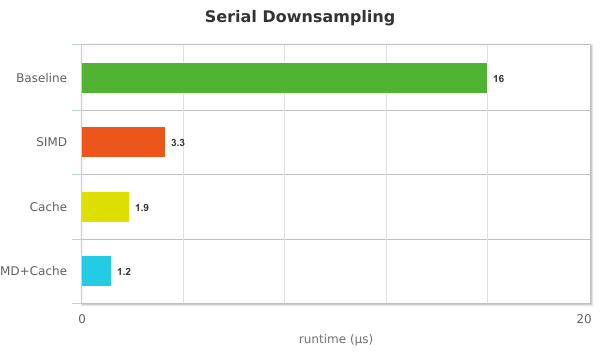
\includegraphics[width=0.9\textwidth]{images/sd}
  \caption{Single-threaded downsampling}
  \end{figure}
\end{frame}

\begin{frame}
  \frametitle{Downsampling}
  \begin{figure}
  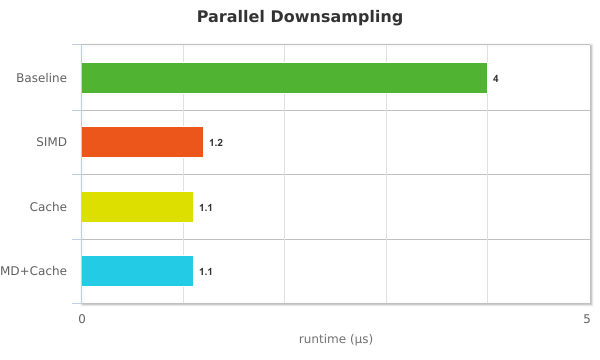
\includegraphics[width=0.9\textwidth]{images/pd}
  \caption{Multi-threaded downsampling}
  \end{figure}
\end{frame}

\begin{frame}
  \frametitle{Bandwith}
  \begin{figure}
  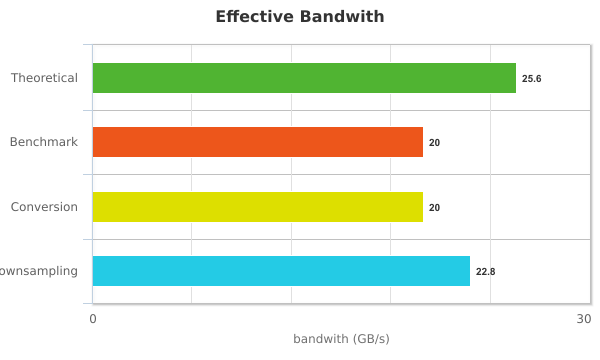
\includegraphics[width=0.9\textwidth]{images/bandwith}
  \caption{Effective Bandwith}
  \end{figure}
\end{frame}

\begin{frame}
  \frametitle{Conclusion}
  \begin{itemize}
    \item{Pay attention to your cache}
    \item{SIMD can be useful even when not compute bound}
    \item{Memory bandwith matters}
    \item{Memory bandwith is hard to optimize for\footnote{http://codearcana.com/posts/2013/05/18/achieving-maximum-memory-bandwidth.html}}
  \end{itemize}
\end{frame}

\end{document}
